\chapter{Background}

Throughout this chapter, let \(n\) be a nonnegative integer.

\section{Permutations and compositions}

The \vocab{symmetric group} \(\sym{n}\) is
the group of all permutations of the set
\(\interval{n} = \{1, 2, \ldots, n\}\).
We write permutations in one-line notation
\(\sigma = \window{\sigma_1, \sigma_2, \ldots, \sigma_n}\).
Given two permutations \(\sigma, \pi \in \sym{n}\),
their product is the permutation \(\sigma \pi \in \sym{n}\)
defined by \((\sigma \pi)_i = \sigma_{\pi_i}\).
The \vocab{reverse} \(\rev(\sigma)\) of
a permutation \(\sigma \in \sym{n}\) is the permutation
\(\rev(\sigma) = \sigma w_0 = \window{\sigma_n, \sigma_{n-1}, \dots, \sigma_1}\),
where \(w_0 = \window{n, n-1, \cdots, 1}\).
The symmetric group \(\sym{n}\) is generated by
the \vocab{simple transpositions} \(s_1, s_2, \ldots, s_{n-1}\),
where \(s_i \in \sym{n}\) is the permutation that swaps the elements \(i\) and \(i+1\) and fixes all other elements.
The \vocab{length} \(\ell(\sigma)\) of a permutation \(\sigma \in \sym{n}\) is
the smallest number of simple transpositions whose product equals \(\sigma\).
A \vocab{reduced expression} of a permutation \(\sigma\) is
a sequence \(s_{i_1},s_{i_2},\ldots,s_{i_{\ell(\sigma)}}\) of simple transpositions
whose product \(s_{i_1}s_{i_2}\cdots s_{i_{\ell(\sigma)}}\) equals \(\sigma\).

A \vocab{composition of length \(n\)} is a sequence
\(\alpha = \composition{\alpha_1, \alpha_2, \ldots, \alpha_n}\)
of nonnegative integers.
A \vocab{partition} is a weakly decreasing composition,
and an \vocab{antipartition} is a weakly increasing composition.
Given a composition \(\alpha\), let \(\dec(\alpha)\) and \(\inc(\alpha)\) denote
the partition and antipartition obtained by sorting the parts of \(\alpha\)
in weakly decreasing and weakly increasing order, respectively.
Define \(\rev(\alpha)=\composition{\alpha_n, \alpha_{n-1}, \ldots, \alpha_1}\)
to be the composition given by reversing the parts of \(\alpha\).

The \vocab{exponent notation} for a composition \(\alpha = \composition{\alpha_1, \ldots, \alpha_n}\)
is given by a sequence of nonnegative integers \(p_1, p_2, \ldots, p_k\)
and positive integers \(m_1, m_2, \ldots, m_k\) that sum to \(n\)
such that \(p_i \neq p_{i+1}\) for \(i\in[k-1]\), written as
\begin{equation*}
	\alpha = \composition{
		\underbrace{p_1 p_1 \ldots p_1}_{m_1},
		\underbrace{p_2 p_2 \ldots p_2}_{m_2},
		\ldots,
		\underbrace{p_k p_k \ldots p_k}_{m_k}
	} = p_1^{m_1} p_2^{m_2} \ldots p_k^{m_k}.
\end{equation*}

Given a permutation \(\pi \in \sym{n}\) and a composition \(\alpha = \composition{\alpha_1, \ldots, \alpha_n}\),
the \vocab{left action} of \(\pi\) on \(\alpha\) is the composition
\(\pi \permact \alpha = \composition{\alpha_{\pi^{-1}(1)}, \alpha_{\pi^{-1}(2)}, \ldots, \alpha_{\pi^{-1}(n)}}\).
In particular,
this choice of notation guarantees that
\(\sigma \permact (\pi \permact \alpha) = (\sigma \pi) \permact \alpha\)
for all \(\sigma, \pi \in \sym{n}\) and
\(\alpha=\composition{\alpha_1,\ldots,\alpha_n}\).
Note that \(\rev(\alpha) = w_0 \permact \alpha\).

\begin{example}
	For example, \(\alpha=\composition{3, 1, 0, 2, 2, 0}\) is
	a composition of length \(6\) with exponent notation \(3^11^10^12^20^1\).
	It rearranges to the partition \(\dec(\alpha) = \composition{3, 2, 2, 1, 0, 0}\),
	the antipartition \(\inc(\alpha) = \composition{0, 0, 1, 2, 2, 3}\),
	and \(\rev(\alpha)=\composition{0,2,1,0,2,3}\).
	The permutation \(\pi = \window{3, 1, 2, 4, 6, 5}\) has reduced expression \(s_2s_1s_5\).
	The result of the left action of \(\pi\) on \(\alpha\) is
	the composition \(\pi \permact \alpha = \composition{1, 0, 3, 2, 0, 2}\),
	with a graphical representation shown in \Cref{fig:left-action-on-composition}.
\end{example}

\begin{figure}[htbp]
    \centering
	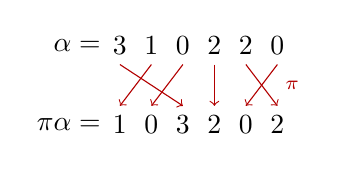
\begin{tikzpicture}[x=.4cm, y=-.5cm]
		\node[anchor=east] at (0.7, 0) {\(\alpha = \)};
		\foreach \i [count = \j] in {3, 1, 0, 2, 2, 0}{
				\node (A\j) at (\j, 0) {\(\i\)};
			}
		\node[anchor=east] at (0.7, 2) {\(\pi \permact \alpha = \)};
		\foreach \i [count = \j] in {1, 0, 3, 2, 0, 2}{
				\node (B\j) at (\j, 2) {\(\i\)};
			}
		\node[anchor=east, color=red!70!black] at (7, 1) {\(\scriptstyle \pi\)};
		\foreach \i [count = \j] in {3, 1, 2, 4, 6, 5}{
				\draw[->, color=red!70!black] (A\j.south) -- (B\i.north);
			}
	\end{tikzpicture}
	\caption{
		The left action of \(\pi = \window{3, 1, 2, 4, 6, 5}\)
		on \(\alpha = \composition{3, 1, 0, 2, 2, 0}\).
		}
	\label{fig:left-action-on-composition}
\end{figure}

\begin{remark}
	Given permutations \(\sigma, \pi \in \sym{n}\) and
	a composition \(\alpha=\composition{\alpha_1,\ldots,\alpha_n}\),
	\cite{Ale19} writes \(\pi \alpha\) to mean \(\pi \permact \alpha\),
	and writes \(\pi \sigma\) to mean \(\pi \permact \sigma\),
	interpreting \(\sigma\) as a composition,
	which we write as a product \(\pi \sigma^{-1}\).
\end{remark}

\section{Algebraic definitions of multiple variations of Macdonald polynomials}

In this section, we define multiple variations of Macdonald polynomials:
\begin{itemize}
    \item \(\tilde{H}_\mu\), the modified Macdonald polynomials,
    \item \(J_\mu\), the integral form symmetric Macdonald polynomials,
    \item \(P_\mu\), the symmetric Macdonald polynomials,
    \item \(E_\alpha^\sigma\), the permuted-basement nonsymmetric Macdonald polynomials,
    \item \(\mathcal{E}_\alpha^\sigma\), the integral form permuted-basement nonsymmetric Macdonald polynomials.
\end{itemize}

\subsection{Modified Macdonald polynomials \texorpdfstring{\(\tilde{H}_\mu\)}{H̃μ}}

\subsection{Integral form symmetric Macdonald polynomials \texorpdfstring{\(J_\mu\)}{Jμ}}

\subsection{Symmetric Macdonald polynomials \texorpdfstring{\(P_\mu\)}{Pμ}}

\subsubsection{Symmetric Macdonald polynomials \texorpdfstring{\(P_\mu\)}{Pμ} as orthogonal polynomials}

\cite{Mac88} 

Define the scalar product \(\langle \cdot, \cdot \rangle_{(q, t)}\) on the ring of symmetric functions with coefficients in \(\rationals(q, t)\) by setting
\begin{equation}
\langle p_\lambda, p_\mu \rangle_{(q, t)} = \delta_{\lambda\mu} z_\lambda(q, t)
\end{equation}
where \(p_\lambda\) is the power sum symmetric function and
\begin{equation}
z_\lambda(q, t) = z_\lambda \prod_{i=1}^{\ell(\lambda)} \frac{1 - q^{\lambda_i}}{1 - t^{\lambda_i}}.
\end{equation}
% If \(q, t\) are treated as real parameters lying in \( (0, 1) \), then the scalar product is positive definite.

\begin{theorem}
	There exists a unique family of symmetric functions \(P_\lambda = P_\lambda(\mathbf{x}; q, t)\) indexed by partitions \(\lambda\) such that:
	\begin{itemize}
	\item \( P_\lambda = m_\lambda + \sum_{\mu < \lambda} u_{\lambda\mu}(q, t) m_\mu \) with coefficients \( u_{\lambda\mu}(q, t) \in \rationals(q, t) \), and;
	\item \( \langle P_\lambda, P_\mu \rangle_{(q, t)} = 0 \quad \text{if } \lambda \ne \mu \).
	\end{itemize}
\end{theorem}

The functions \(P_\lambda\) are called the \vocab{symmetric Macdonald polynomials}.

\subsubsection{Symmetric Macdonald polynomials \texorpdfstring{\(P_\mu\)}{Pμ} as eigenfunctions}

\cite{Mac88} 

For any polynomial \( f(x_1, \ldots, x_n) \) and \(1 \le i \le n\), define the \(q\)-shift operator \(T_{q,x_i}\) by
\begin{equation}
(T_{q,x_i} f)(x_1, \ldots, x_n) = f(x_1, \ldots, qx_i, \ldots, x_n).
\end{equation}
Then, the operator \( D \) is defined as
\begin{equation}
D = \sum_{i=1}^n \left( \prod_{j \ne i} \frac{t x_i - x_j}{x_i - x_j} \right) T_{q,x_i}.
\end{equation}
The operator \(D\) has distinct eigenfunction, and these eigenfunctions are the symmetric Macdonald polynomials \(P_\lambda(x_1, \ldots, x_n; q, t)\) where \(\lambda\) is a partition with at most \(n\) parts.

\subsection{Permuted-basement Macdonald polynomials \texorpdfstring{\(E_\alpha^\sigma\)}{Eασ} as eigenfunctions}
\label{sec:permuted basement def}

We follow the exposition of \cite{Fer11} and the notation of \cite{Ale19}
for the definition of nonsymmetric Macdonald polynomials
and permuted-basement Macdonald polynomials.
For more background on this topic, see \cite{GR22},
where these polynomials are referred to as the \emph{relative Macdonald polynomials}.

Let \(x_1\), \dots, \(x_n\) be indeterminates, denoted collectively as \(\mathbf{x}\).
Let \(q, t\) be parameters.
We define nonsymmetric Macdonald polynomials and permuted-basement Macdonald polynomials,
which are polynomials in the ring \(\rationals(q, t)[\mathbf{x}]\).

A permutation \(\sigma \in \sym{n}\) acts on
a polynomial \(f(\mathbf{x})\) by permuting the variables,
that is,
\(\sigma (\mathbf{x}^{\alpha}) = \mathbf{x}^{\sigma \permact \alpha}\)
for a composition \(\alpha\).
For example, the permtutation \(\sigma = \window{2, 3, 1}\) sends the monomial \(x_1^2 x_2 = \mathbf{x}^{\composition{2, 1, 0}}\) to the monomial
\begin{equation*}
    \window{2, 3, 1} (x_1^2 x_2)
    = \window{2, 3, 1}(\mathbf{x}^{\composition{2, 1, 0}})
    = \mathbf{x}^{\window{2, 3, 1} \permact \composition{2, 1, 0}}
    = \mathbf{x}^{\composition{0, 2, 1}}
    = x_2^2 x_3.
\end{equation*}

The \vocab{Demazure--Lusztig operators}
\(T_1\), \dots, \(T_{n-1}\) on \(\rationals(q, t)[\mathbf{x}]\)
are defined by
\begin{equation*}
	T_i(f) = ts_i(f) + (1-t) x_{i+1} \frac{f - s_i(f)}{x_i - x_{i+1}},
\end{equation*}
for \(i \in \interval{n-1}\),
and the operator \(g\) on \(\rationals(q, t)[\mathbf{x}]\) is defined by
\begin{equation*}
	g(f(x_1, \ldots, x_n)) = f(x_2, x_3, \ldots, x_n, q^{-1}x_1).
\end{equation*}
For a reduced expression \( \sigma = s_{i_1} \cdots s_{i_k} \),
we write \(T_\sigma\) to denote the composition \(T_{i_1} \circ \cdots \circ T_{i_k}\).
The \vocab{Cherednik--Dunkl operators}
\(Y_1\), \dots, \(Y_n\) on \(\rationals(q, t)[\mathbf{x}]\)
are defined by,
for each \(i \in \interval{n}\),
\begin{equation*}
	Y_i = t^{i-1} T_{i-1}^{-1} \cdots T_1^{-1} g T_{n-1} \cdots T_i.
\end{equation*}

\begin{definition}[{\cite[Theorem 4.1.4]{Fer11}}]
	For a composition \(\alpha=\composition{\alpha_1,\ldots,\alpha_n}\),
	the \vocab{nonsymmetric Macdonald polynomial} \(E_\alpha=E_\alpha(\mathbf{x}; q, t)\) is
	the unique element of \(\rationals(q, t)[\mathbf{x}]\) such that
	the coefficient of \(\mathbf{x}^{\alpha}\) is \(1\),
	and for all \(i\in\interval{n}\),
	\begin{equation*}
		Y_i E_\alpha = q^{-\alpha_i} t^{k_i} E_\alpha,
	\end{equation*}
	where
	\(
		k_i = |\{ j \in \interval{i-1} \suchthat \alpha_j > \alpha_i \}|
			+ |\{ j \in \interval{i+1, n} \suchthat \alpha_j \geq \alpha_i \}|
	\).
\end{definition}

\begin{remark}
	We note that there is a typo in \cite{Fer11}:
	the corresponding formula for \(k_i\) has a minus sign instead of a plus sign.
	Our formulation aligns with the definition in \cite{Kno97},
	although the notation there differs.
\end{remark}

\begin{example}
	\label{example:nonsymmetric-macdonald-polynomial}
	Let \(n = 4\) and \(\alpha = \composition{1, 0, 1, 1}\).
	Then, \(k_1 = 2\), \(k_2 = 3\), \(k_3 = 1\) and \(k_4 = 0\).
	Therefore, the nonsymmetric Macdonald polynomial
	\(E_{\composition{1, 0, 1, 1}}(\mathbf{x}; q, t)\)
	is the unique element of \(\rationals(q, t)[x_1, x_2, x_3, x_4]\) such that
	the coefficient of \(x_1 x_3 x_4\) is \(1\), and
	\begin{align*}
		Y_1 E_{\composition{1, 0, 1, 1}} & = q^{-1} t^{2} E_{\composition{1, 0, 1, 1}}, &
		Y_2 E_{\composition{1, 0, 1, 1}} & = q^{0}  t^{3} E_{\composition{1, 0, 1, 1}}, \\
		Y_3 E_{\composition{1, 0, 1, 1}} & = q^{-1} t^{1} E_{\composition{1, 0, 1, 1}}, &
		Y_4 E_{\composition{1, 0, 1, 1}} & = q^{-1} t^{0} E_{\composition{1, 0, 1, 1}}.
	\end{align*}
	The unique polynomial satisfying the above is
	\begin{equation*}
		E_{\composition{1, 0, 1, 1}}(x_1, x_2, x_3, x_4; q, t)
		=
		x_1 x_2 x_3 \frac{1 - t}{1 - q t^2} +
		x_1 x_2 x_4 \frac{1 - t}{1 - q t^2} +
		x_1 x_3 x_4.
	\end{equation*}
\end{example}

The following definition is a reformulation based on \cite[Corollary 16]{Ale19} and \cite[Remark 4.4.5]{Fer11}.

\begin{definition}[Permuted-basement Macdonald polynomials]
	\label{definition:permutedbasement}
	For a composition \(\alpha=\composition{\alpha_1,\ldots,\alpha_n}\)
	and a permutation \(\sigma \in \sym{n}\),
	the \vocab{permuted-basement Macdonald polynomial}
	\(E_\alpha^\sigma = E_{\alpha}^{\sigma}(\mathbf{x}; q, t)\)
	is given by
	\begin{equation*}
		E_{\alpha}^{\sigma} =
		t^{-\twinv(\alpha, \sigma)} T_{\rev(\sigma)} E_{\rev(\alpha)},
	\end{equation*}
	where
	\(
		\twinv(\alpha, \sigma) =
		\left| \{
			(i, j) \suchthat
			i < j \text{ and }
			\alpha_i \geq \alpha_j \text{ and }
			\sigma_i < \sigma_j
		\} \right|
	\).
\end{definition}

Note that, for \(\sigma = w_0 = \window{n, n-1, \ldots, 1}\),
the permuted-basement Macdonald polynomial \(E_{\alpha}^{w_0}(\mathbf{x}; q, t)\)
is the nonsymmetric Macdonald polynomial \(E_{\rev(\alpha)}(\mathbf{x}; q, t)\).

\begin{remark}
	We note a typo in \cite{Ale19} concerning the definition of \(\twinv(\alpha, \sigma)\):
	the inequality involving \(\sigma\) is reversed.
	This error becomes apparent by considering the special case \(E_\alpha^{w_0}\).
	Our formulation aligns with the definition provided in \cite{Fer11},
	although we use different notation.
\end{remark}

\begin{remark}
	\label{remark:notation-permuted-basement-macdonald-polynomial-Ale19}
	Our notation for the permuted-basement Macdonald polynomial agrees with
	the notation in \cite{Ale19,CMW22},
	which is different from the notation in \cite{Fer11}.
	Notably, the permuted-basement Macdonald polynomial \(E_{\alpha}^{\sigma}(\mathbf{x}; q, t)\)
	is denoted by \(E_{\rev(\alpha)}^{\rev(\sigma)}(\mathbf{x};q,t)\) in \cite{Fer11}.
\end{remark}

\begin{example}
	\label{example:permuted-basement-macdonald-polynomial}
	Let \(n = 4\),
	\(\alpha = \composition{1, 1, 0, 1}\),
	and \(\sigma = \window{2, 4, 1, 3}\).
	Then, \(\rev(\sigma)=\window{3, 1, 4, 2}\) has reduced expression \(s_2 s_1 s_3\),
	so the Demazure--Lusztig operator \(T_{\rev(\sigma)}\) is given by \(T_2 T_1 T_3\).
	We compute
	\(
		\twinv(\alpha, \sigma) =
		\twinv(\composition{1, 1, 0, 1}, \window{2, 4, 1, 3}) =
		|\{(1, 2), (1, 4)\}| = 2
	\).
	Therefore,
	the permuted-basement Macdonald polynomial
	\(E_{\composition{1, 1, 0, 1}}^{\window{2, 4, 1, 3}}(\mathbf{x}; q, t)\)
	is given by
	\begin{equation*}
		E_{\composition{1, 1, 0, 1}}^{\window{2, 4, 1, 3}}(\mathbf{x}; q, t)
		=
		t^{-2}
		T_2 T_1 T_3
		E_{\composition{1, 0, 1, 1}}(\mathbf{x}; q, t),
	\end{equation*}
	which can be computed from \cref{example:nonsymmetric-macdonald-polynomial} as
	\begin{equation*}
		E_{\composition{1, 1, 0, 1}}^{\window{2, 4, 1, 3}}
		=
		x_{1} x_{2} x_{3} \frac{t(1 - t)}{1 - q t^2} +
		x_{1} x_{3} x_{4} \frac{1 - t}{1 - q t^2} +
		x_{2} x_{3} x_{4}.
	\end{equation*}
\end{example}

\begin{example}
	Let \(n = 4\),
	\(\alpha = \composition{1, 1, 0, 1}\),
	and \(\tau = \window{4, 2, 1, 3}\).
	Then, \(\rev(\tau) = \window{3, 1, 4, 2}\) has a reduced expression \(\rev(\tau) = s_2 s_1\),
	so the Demazure--Lusztig operator \(T_{\rev(\tau)}\) is given by \(T_2 T_1\).
	We compute
	\(
		\twinv(\alpha, \tau) =
		\twinv(\composition{1, 1, 0, 1}, \window{4, 2, 1, 3}) =
		|\{(1, 4)\}| = 1
	\).
	Therefore, the permuted-basement Macdonald polynomial
	\(E_{\composition{1, 1, 0, 1}}^{\window{4, 2, 1, 3}}(\mathbf{x}; q, t)\)
	is given by
	\begin{equation*}
		E_{\composition{1, 1, 0, 1}}^{\window{4, 2, 1, 3}}(\mathbf{x}; q, t)
		=
		t^{-1}
		T_2 T_1
		E_{\composition{1, 0, 1, 1}}(\mathbf{x}; q, t),
	\end{equation*}
	which can be computed as
	\begin{equation*}
		E_{\composition{1, 1, 0, 1}}^{\window{4, 2, 1, 3}}
		=
		x_{1} x_{2} x_{3} \frac{t(1 - t)}{1 - q t^2} +
		x_{1} x_{3} x_{4} \frac{1 - t}{1 - q t^2} +
		x_{2} x_{3} x_{4}.
	\end{equation*}
\end{example}

\subsection{Integral form permuted-basement Macdonald polynomials \texorpdfstring{\(\mathcal{E}_\alpha^\sigma\)}{Eασ}}

\section{Combinatorial formulas for multiple variations of Macdonald polynomials}

\subsection{Unsigned and Signed Alphabets}

An \vocab{unsigned alphabet} \(\mathcal{A}\) is a totally ordered set.
We write \(\ind{a, b}\) to denote the indicator function of \(a > b\).
Usually, we take \(\mathcal{A} = [n]\) or \(\mathcal{A} = \positives\).

A \vocab{signed alphabet} \(\mathcal{A}_\pm\) is a total oder on the disjoint union of two copies of a set \(\mathcal{A}\), a \vocab{positive} copy \(\mathcal{A}_+\) and a \vocab{negative} copy \(\mathcal{A}_-\).
We write \(\ind{a, b}\) to denote the indicator function of \(a > b\) or \(a = b \in \mathcal{A}_-\).
Given an element \(a \in \mathcal{A}\), we denote its positive copy by \(a \in \mathcal{A}_+\) and its negative copy by \(\bar{a} \in \mathcal{A}_-\),
and we say that \(a \in \mathcal{A}\) is the \vocab{absolute value} of \(a \in \mathcal{A}_+\) and \(\bar{a} \in \mathcal{A}_-\), denoted \(|a| = |\bar{a}| = a\).
Some signed alphabets we use are \(\integers_\pm\), with the total order
\begin{equation*}
	1 < \bar{1} < 2 < \bar{2} < 3 < \bar{3} < \cdots,
\end{equation*}
and its subalphabet \([n]_\pm\).

In both unsigned and signed alphabets,
\begin{equation*}
	\ind{a, b, c} = \ind{a, b} + \ind{b, c} - \ind{a, c}.
\end{equation*}
We have \(\ind{a, b, c} \in \{0, 1\}\) since it is impossible for \(\ind{a, b} = \ind{b, c} = 1 - \ind{a, c}\).

We will also use the symbol \(\infty\) to denote an element larger than any element in \(\mathcal{A}\), so that \(\ind{a, \infty} = 1\) and \(\ind{\infty, a} = 0\) for all \(a \in \mathcal{A}\).
Note that \(\infty\) is not an element of \(\mathcal{A}\).

Here's one way to think about \(\ind{a, b, c}\).
For an unsigned alphabet,
\(\ind{a, b, c}\) indicates whether \(a, b, c\) is cyclically weakly decreasing, where the earlier of two equal entries is considered smaller than the later one.
That is, in an unsigned alphabet,
\(\ind{a, b, c} = 1\) if and only if
\begin{equation*}
	a > b > c \quad \text{or} \quad b > c \geq a \quad \text{or} \quad c \geq a > b.
\end{equation*}
\Cref{fig:indicator} provides examples of the indicator function \(\ind{a, b, c}\).

\begin{figure}[htbp]
	\centering
	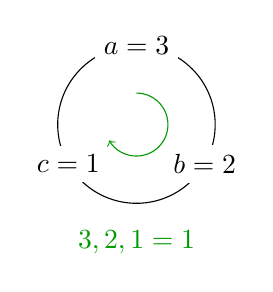
\begin{tikzpicture}
		\draw[black] (0, 0) circle (1);
		\node[rectangle, fill=white] at (90:1) {\(a = 3\)};
		\node[rectangle, fill=white] at (-30:1) {\(b = 2\)};
		\node[rectangle, fill=white] at (-150:1) {\(c = 1\)};
		\draw[->, green!60!black] (90:.4) arc (90:-150:.4);
		\node[green!60!black] at (0, -1.5) {\(\ind{3, 2, 1} = 1\)};
	\end{tikzpicture} \hspace{1cm}
	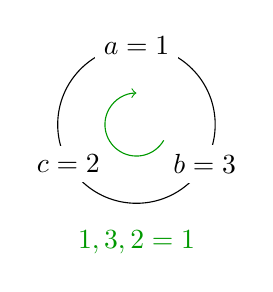
\begin{tikzpicture}
		\draw[black] (0, 0) circle (1);
		\node[rectangle, fill=white] at (90:1) {\(a = 1\)};
		\node[rectangle, fill=white] at (-30:1) {\(b = 3\)};
		\node[rectangle, fill=white] at (-150:1) {\(c = 2\)};
		\draw[->, green!60!black, rotate=-120] (90:.4) arc (90:-150:.4);
		\node[green!60!black] at (0, -1.5) {\(\ind{1, 3, 2} = 1\)};
	\end{tikzpicture} \hspace{1cm}
	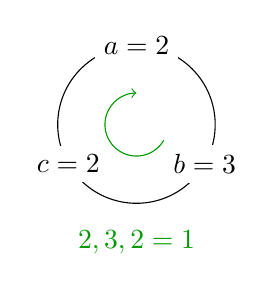
\begin{tikzpicture}
		\draw (0, 0) circle (1);
		\node[rectangle, fill=white] at (90:1) {\(a = 2\)};
		\node[rectangle, fill=white] at (-30:1) {\(b = 3\)};
		\node[rectangle, fill=white] at (-150:1) {\(c = 2\)};
		\draw[->, green!60!black, rotate=-120] (90:.4) arc (90:-150:.4);
		\node[green!60!black] at (0, -1.5) {\(\ind{2, 3, 2} = 1\)};
	\end{tikzpicture} \\
	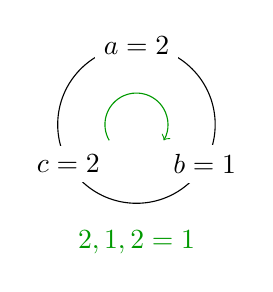
\begin{tikzpicture}
		\draw[black] (0, 0) circle (1);
		\node[rectangle, fill=white] at (90:1) {\(a = 2\)};
		\node[rectangle, fill=white] at (-30:1) {\(b = 1\)};
		\node[rectangle, fill=white] at (-150:1) {\(c = 2\)};
		\draw[->, green!60!black, rotate=120] (90:.4) arc (90:-150:.4);
		\node[green!60!black] at (0, -1.5) {\(\ind{2, 1, 2} = 1\)};
	\end{tikzpicture} \hspace{1cm}
	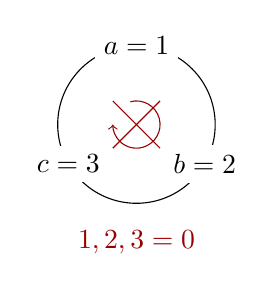
\begin{tikzpicture}
		\draw[black] (0, 0) circle (1);
		\node[rectangle, fill=white] at (90:1) {\(a = 1\)};
		\node[rectangle, fill=white] at (-30:1) {\(b = 2\)};
		\node[rectangle, fill=white] at (-150:1) {\(c = 3\)};
		\draw[->, red!60!black] (105:.3) arc (105:-180:.3);
		\draw[red!60!black] (.3,.3) -- (-.3,-.3);
		\draw[red!60!black] (.3,-.3) -- (-.3,.3);
		\node[red!60!black] at (0, -1.5) {\(\ind{1, 2, 3} = 0\)};
	\end{tikzpicture} \hspace{1cm}
	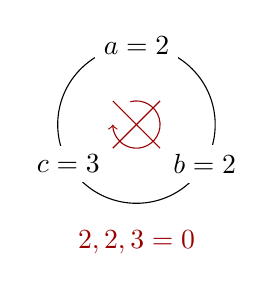
\begin{tikzpicture}
		\draw[black] (0, 0) circle (1);
		\node[rectangle, fill=white] at (90:1) {\(a = 2\)};
		\node[rectangle, fill=white] at (-30:1) {\(b = 2\)};
		\node[rectangle, fill=white] at (-150:1) {\(c = 3\)};
		\draw[->, red!60!black] (105:.3) arc (105:-180:.3);
		\draw[red!60!black] (.3,.3) -- (-.3,-.3);
		\draw[red!60!black] (.3,-.3) -- (-.3,.3);
		\node[red!60!black] at (0, -1.5) {\(\ind{2, 2, 3} = 0\)};
	\end{tikzpicture}
	\caption{Examples of the indicator function \(\ind{a, b, c}\).}
	\label{fig:indicator}
\end{figure}

In signed alphabets, \(\ind{a, b, c}\) indicates whether \(a, b, c\) is cyclically decreasing, where the earlier of two equal positive entries is considered smaller than the later one, and the earlier of two equal negative entries is considered larger than the later one.

\subsection{Non-augmented Fillings} \label{subsec:non-augmented-fillings}

The \vocab{(non-augmented) skyline diagram} of a composition
\(\alpha = \composition{\alpha_1, \ldots, \alpha_n}\)
is the set
\begin{equation*}
	\dg(\alpha) = \left\{ (i, r) \suchthat i \in \interval{n} \text{ and } r \in \interval{\alpha_i} \right\},
\end{equation*}
where the first coordinate indexes the columns and the second coordinate indexes the rows.
In \cref{subsec:augmented-fillings}, we will define the \vocab{augmented skyline diagram} of a composition, hence the optional term \emph{non-augmented} is used when the distinction is necessary.
The elements of \(\dg(\alpha)\) are called \vocab{boxes}.
We draw the box \((i, r)\) as a square in column \(i\) and row \(r\).
\Cref{fig:skyline} provides an example of a skyline diagram.

\begin{figure}[htbp]
	\centering
	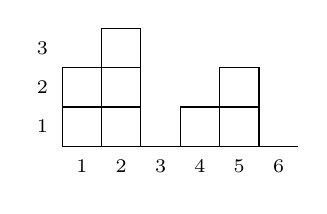
\begin{tikzpicture}[x=.5cm, y=.5cm]
		\foreach \height [count = \column] in {2, 3, 0, 1, 2, 0}{
				\foreach \row in {0,...,\height}{
						\ifnum \row = 0
							\path (\column, \row) rectangle (\column + 1, \row + 1);
							\draw (\column, \row+1) -- (\column + 1, \row + 1);
						\else
							\draw[black] (\column, \row) rectangle (\column + 1, \row + 1);
						\fi
					}
				\node at (\column + .5, .5) {\(\scriptstyle \column\)};
			}
		\foreach \row in {1, 2, 3}{
				\node at (.5, \row + .5) {\(\scriptstyle \row\)};
			}
	\end{tikzpicture}
	\caption{
		The skyline diagram 
		of the composition \(\alpha = \composition{2, 3, 0, 1, 2, 0}\).
	}
	\label{fig:skyline}
\end{figure}

A box \(u = (i_u, r_u)\) \vocab{attacks} \(v = (i_v, r_v)\) in \(\dg(\alpha)\) if
\(r_u = r_v\) and \(i_u < i_v\), that is, \(u\) and \(v\) are in the same row and \(u\) is to the left of \(v\); or
\(r_v = r_u - 1\) and \(i_v < i_u\), that is, \(u\) is in the row directly above \(v\) and \(u\) is to the right of \(v\).
\Cref{fig:attacking} illustrates the two configurations in which a box \(u\) attacks a box \(v\).
Let \(\Attack(u) \subset \dg(\alpha)\) be the set of boxes attacked by \(u\).

\begin{figure}[htbp]
	\begin{equation*}
		\vcenter{\hbox{
				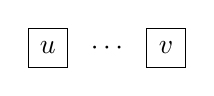
\begin{tikzpicture}[x=.5cm, y=.5cm]
					\draw[black] (0, 0) rectangle (1, 1);
					\node at (.5, .5) {\(u\)};
					\node at (2, .5) {\(\cdots\)};
					\draw[black] (3, 0) rectangle (4, 1);
					\node at (3.5, .5) {\(v\)};
				\end{tikzpicture}}}
		\qquad \text{or} \qquad
		\vcenter{\hbox{
				\begin{tikzpicture}[x=.5cm, y=.5cm]
					\draw[black, shift={(0,-.5)}] (0, 0) rectangle (1, 1);
					\node at (.5, .5-.5) {\(v\)};
					\node at (2, .5) {\(\cdots\)};
					\draw[black, shift={(0,.5)}] (3, 0) rectangle (4, 1);
					\node at (3.5, .5+.5) {\(u\)};
				\end{tikzpicture}}}.
	\end{equation*}
	\caption{Configurations in which a box \(u\) attacks a box \(v\): either in the same row (left), or in consecutive rows (right). }
	\label{fig:attacking}
\end{figure}

Let \(u = (i, r) \in \dg(\alpha)\).
The \vocab{leg set} of \(u\) is the set \(\Leg(u) \subset \dg(\alpha)\) of boxes above \(u\) in the same column, that is, \(\Leg(u) = \left\{ (i, r') \in \dg(\alpha) \suchthat r' > r \right\}\).
The \vocab{leg statistic} of \(u\) is defined as \(\leg(u) = \left|\Leg(u)\right| = \alpha_i - r\).
The \vocab{arm set} of \(u\) is the set \(\Arm(u) \subset \dg(\alpha)\) of boxes \(v\) attacked by \(u\) such that \(\leg(v) \leq \leg(u)\), that is,
\begin{equation*}
	\Arm(u) = \left\{ v \in \Attack(u) \suchthat \leg(v) \leq \leg(u) \right\}.
\end{equation*}
The \vocab{arm statistic} of \(u\) is defined as \(\arm(u) = \left|\Arm(u)\right|\).
The box \vocab{south} of \(u = (i, r)\) is the box \(\south{u} = (i, r-1)\), that is, the box directly below \(u\).
If \(r > 1\), then \(\south{u} \in \dg(\alpha)\); while if \(r = 1\), then \(\south{u}\) is still defined (in row \(0\)),
but it is not in \(\dg(\alpha)\).
See \cref{fig:leg-arm} for an example of the leg set, arm set, and south of a box.

\begin{figure}[htbp]
    \centering
	\begin{tikzpicture}[x=.5cm, y=.5cm]
		\def\shape{3, 2, 2, 4, 4, 0, 3, 3, 3, 4, 2, 1, 3}
		\xdef\reading{0}
		\foreach \height [count = \column] in \shape{
			\foreach \row in {0,...,\height}{
					\pgfmathparse{int(\reading + 1)}
					\xdef\reading{\pgfmathresult}
					\coordinate (B\reading) at (\column, \row);
				}
		}
		\def\filling{
			{ },{ },{ },{ },
			{ },{z},{ },
			{ },{z},{ },
			{ },{ },{ },{ },{ },
			{ },{ },{ },{ },{ },
			{ },
			{ },{ },{ },{ },
			{ },{d},{u},{x},
			{ },{ },{z},{ },
			{ },{ },{ },{ },{ },
			{ },{ },{z},
			{ },{ },
			{ },{ },{z},{ }}

		\foreach \i [count = \j] in \filling {
			\if\i u
				\draw[fill=black] (B\j) rectangle ++(1, 1);
			\else\if\i z
					\draw[pattern color=magenta, pattern=north east lines] (B\j) rectangle ++(1, 1);
				\else\if\i x
						\draw[pattern color=green!70!black, pattern=vertical lines] (B\j) rectangle ++(1, 1);
					\else\if\i d
							\draw[pattern color=yellow!50!black, pattern=horizontal lines] (B\j) rectangle ++(1, 1);
						\else
							\draw[fill=white] (B\j) rectangle ++(1, 1);
						\fi\fi\fi\fi
		}

	\end{tikzpicture}
	\caption{
		The leg set (\,\raisebox{-.7ex}{\begin{tikzpicture}[x=.45cm, y=.45cm] \protect\draw[pattern color=green!70!black, pattern=vertical lines] (0, 0) rectangle ++(1, 1); \end{tikzpicture}}\,),
		the arm set (\,\raisebox{-.7ex}{\begin{tikzpicture}[x=.45cm, y=.45cm] \protect\draw[pattern color=magenta, pattern=north east lines] (0, 1) rectangle ++(1, 1); \end{tikzpicture}}\,),
		and the south (\,\raisebox{-.7ex}{\begin{tikzpicture}[x=.45cm, y=.45cm] \protect\draw[pattern color=yellow!50!black, pattern=horizontal lines] (1, 4) rectangle ++(1, 1); \end{tikzpicture}}\,)
		of a box \(u = (8, 3)\) (\,\raisebox{-.7ex}{
\begin{tikzpicture}[x=.45cm, y=.45cm] \protect\draw[fill=black] (5, 2) rectangle ++(1, 1); \end{tikzpicture}}\,)
		in the skyline diagram of \(\alpha = \composition{4, 3, 3, 5, 5, 1, 4, 4, 4, 5, 3, 2, 4}\) with \(\leg(u)=1\) and \(\arm(u)=5\).
	}
	\label{fig:leg-arm}
\end{figure}

A \vocab{filling} of shape \(\alpha = \composition{\alpha_1, \ldots, \alpha_n}\) with labels in an alphabet \(\mathcal{A}\) is a function \(T \colon \dg(\alpha) \to \mathcal{A}\).
Let \(\Fill[\mathcal{A}](\alpha)\) denote the set of fillings of shape \(\alpha\) with labels in \(\mathcal{A}\).
A filling \(T\in \Fill[\mathcal{A}](\alpha)\)
is \vocab{non-attacking} if \(T(u_1) \neq T(u_2)\) for all pairs of attacking boxes \(u_1\) and \(u_2\) in \(\dg(\alpha)\).
Let \(\NAF[\mathcal{A}](\alpha) \subseteq \Fill[\mathcal{A}](\alpha)\) denote the set of non-attacking fillings of shape \(\alpha\) with labels in \(\mathcal{A}\).

The \vocab{content} of a filling \(T\) with labels in the unsigned alphabet \(\mathcal{A} = \interval{n}\) or \(\mathcal{A} = \positives\) is the composition \(\beta = \content(T)\) where \(\beta_i\) is the number of occurrences of the label \(i\) in \(T\).
The \vocab{content} of a filling \(T\) with labels in the signed alphabet \(\mathcal{A}_\pm = [n]_\pm\) or \(\mathcal{A}_\pm = \integers_\pm\) is the composition \(\beta = \content(T)\) where \(\beta_i\) is the number of occurrences of the label \(i\) or \(\bar{i}\) in \(T\).
In both contexts, we let
\[
	\mathbf{x}^T = \mathbf{x}^{\content(T)} = \prod_{i} x_i^{\beta_i}.
\]

See \Cref{fig:non-attacking-filling} for an example of a non-attacking filling.

\begin{figure}[htbp]
    \centering
	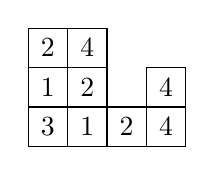
\begin{tikzpicture}[x=.5cm, y=.5cm]
		\def\shape{2, 2, 0, 1}
		\def\filling{
			3, 1, 2,
			1, 2, 4,
			2,
			4, 4}
		\edef\reading{0}
		\foreach \height [count = \column] in \shape{
			\foreach \row in {0,...,\height}{
					\pgfmathparse{int(\reading + 1)}
					\xdef\reading{\pgfmathresult}
					\draw[black] (\column, \row) rectangle (\column + 1, \row + 1);
					\coordinate (B\reading) at (\column + .5, \row + .5);
				}
		}
		\foreach \i [count = \j] in \filling{ \node at (B\j) {\i}; }
	\end{tikzpicture}
	\caption{
		A non-attacking filling of
		shape \(\alpha = \composition{3, 3, 1, 2}\)
		with \(\content(T) = \composition{2, 3, 1, 3}\).
	}
	\label{fig:non-attacking-filling}
\end{figure}

Recall that boxes in row \(0\), which are not in \(\dg(\alpha)\),
can be obtained as the south of boxes in row \(1\).
By convention, if \(w\) is a box in row \(0\),
then we define \(T(w) = \infty\).

Given a filling \(T \in \Fill(\alpha)\),
we say that a box \(u \in \dg(\alpha)\)
is a \vocab{descent} in \(T\) if \(\ind{T(u), T(\south{u})} = 1\).
Note that boxes in row \(1\) are never descents,
since the label of the south of a box in row \(1\) is always \(\infty\), by convention.
Let \(\Des(T) \subseteq \dg(\alpha)\) denote the set of descents in \(T\).
The \vocab{major index} of \(T\) is
\begin{equation*}
	\maj(T)
	= \sum_{u \in \Des(T)} \left( \leg(u) + 1 \right)
	= \sum_{u \in \dg(\alpha)} \ind{T(u), T(\south{u})} \left( \leg(u) + 1 \right).
\end{equation*}
See \cref{fig:major-index} for an example.
\begin{figure}[htbp]
    \centering
	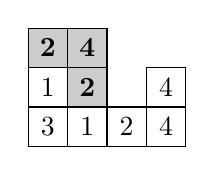
\begin{tikzpicture}[x=.5cm, y=.5cm]
		\def\shape{2, 2, 0, 1}
		\def\filling{
			3, 1, \textbf2,
			1, \textbf2, \textbf4,
			2,
			4, 4}
		\xdef\reading{0}
		\fill[black!20] (1,2) rectangle ++(1,1);
		\fill[black!20] (2,1) rectangle ++(1,1);
		\fill[black!20] (2,2) rectangle ++(1,1);
		\foreach \height [count = \column] in \shape{
			\foreach \row in {0,...,\height}{
					\pgfmathparse{int(\reading + 1)}
					\xdef\reading{\pgfmathresult}
					\draw[black] (\column, \row) rectangle (\column + 1, \row + 1);
					\coordinate (B\reading) at (\column + .5, \row + .5);
				}
		}
		\foreach \i [count = \j] in \filling{
			\node at (B\j) {\i};
		}
	\end{tikzpicture}
	\caption{
		The filling \(T\) above has three descents (shaded boxes).
		The leg statistics of the descents are: \(\leg(1,2)=\leg(2,2)=0\) and \(\leg(2,1)=1\).
		Thus, the major index of \(T\) is \(\maj(T) = 1 + 1 + 2 = 4\).
	}
	\label{fig:major-index}
\end{figure}

A \vocab{triple} is an ordered tuple \((u, v, w)\) of boxes
such that \(u \in \dg(\alpha)\), \(v \in \Arm(u)\), and \(w = \south{u}\).
If \(v\) is to the right of \(u\) in the same row as \(u\),
then the triple is of \vocab{type A},
and if \(v\) is to the left of \(u\) in the row directly below \(u\),
then the triple is of \vocab{type B}.%
\footnote{This is not related to Cartan types \(A_n\) and \(B_n\). They are called \vocab{type II} and \vocab{type I}, respectively, in \cite{HHL08} and \cite{Fer11}.}
The configurations of the boxes \(u\), \(v\), and \(w\)
when the tuple \((u, v, w)\) is of type A or type B are shown in \cref{fig:triples}.
Note that if \(\alpha\) is a partition, there are no triples of type B.
\begin{figure}[ht]
	\centering
	\begin{subfigure}[t]{0.45\textwidth}
		\centering
		\begin{ytableau}
			u & \none[\cdots] & v \\
			w
		\end{ytableau}
		\caption*{(\textsc{Type A})
		The column containing \(u\) and \(w\) is at least as high as the column containing \(v\).}
	\end{subfigure}\hspace{0.05\textwidth}
	\begin{subfigure}[t]{0.45\textwidth}
		\centering
		\begin{ytableau}
			\none & \none & u \\
			v & \none[\cdots] & w
		\end{ytableau}
		\caption*{(\textsc{Type B})
		The column containing \(u\) and \(w\) is strictly higher than the column containing \(v\).}
	\end{subfigure}
	\caption{Configurations for triples of type A (left) and type B (right).}
	\label{fig:triples}
\end{figure}

Note that the definition of a triple \((u, v, w)\) allows for \(u\) to be in row \(1\), and consequently for \(w\) to be in row \(0\).
A triple that has \(u\) in row \(1\) is called a \vocab{degenerate triple}.
A degenerate triple is always of type A, since \(v \in \Arm(u) \subset \dg(\alpha)\), and therefore cannot be in row \(0\).

% We define the \vocab{inversion} and \vocab{coinversion} statistics,
% following \cite[Section~3]{HHL08}.

Given a filling \(T \in \Fill(\alpha)\),
a triple \((u, v, w)\) in \(\dg(\alpha)\) is
an \vocab{inversion triple} if \(\ind{T(u), T(v), T(w)} = 1\),
and is a \vocab{coinversion triple} otherwise.
Let \(\inv(T)\) and \(\coinv(T)\) denote
the number of inversion triples and coinversion triples in \(T\),
respectively.
% It is straightforward to check that these definitions of inversion triples
% are equivalent to those in \cite{Ale19} and \cite{CMW22}.
See \cref{fig:inversion-coinversion} for an example.

\begin{figure}[htbp]
    \centering
	\ytableausetup{boxsize=0.5cm}
	\colorlet{inversion}{orange!70!white}
	\colorlet{coinversion}{purple!50!white}
	\renewcommand{\arraystretch}{1.5}
	\begin{tabular}{ccccc}
		\begin{ytableau}
			*(coinversion) \textbf2 & *(coinversion) \textbf4 \\
			*(coinversion) \textbf1 & 2 & \none & 4 \\
			3 & 1 & 2 & 4
		\end{ytableau}
		&
		\begin{ytableau}
			2 & 4 \\
			*(coinversion) \textbf1 & *(coinversion) \textbf2 & \none & 4 \\
			*(coinversion) \textbf3 & 1 & 2 & 4
		\end{ytableau}
		&
		\begin{ytableau}
			2 & 4 \\
			*(inversion) \textbf1 & 2 & \none & *(inversion) \textbf4 \\
			*(inversion) \textbf3 & 1 & 2 & 4
		\end{ytableau}
		&
		\begin{ytableau}
			2 & 4 \\
			1 & *(coinversion) \textbf2 & \none & *(coinversion) \textbf4 \\
			3 & *(coinversion) \textbf1 & 2 & 4
		\end{ytableau}
		&
		\begin{ytableau}
			2 & 4 \\
			1 & 2 & \none & *(inversion) \textbf4 \\
			3 & 1 & *(inversion) \textbf2 & *(inversion) \textbf4
		\end{ytableau}
		\\
		\(\ind{2, 4, 1} = 0\)
		&
		\(\ind{1, 2, 3} = 0\)
		&
		\(\ind{1, 4, 3} = 1\)
		&
		\(\ind{2, 4, 1} = 0\)
		&
		\(\ind{4, 2, 1} = 1\)
	\end{tabular}
	\caption{
		We show all five triples of
		the filling \(T\) in \cref{fig:non-attacking-filling};
		the first four are of type A, and the last one is of type B.
		There are two inversion triples (orange)
		and three coinversion triples (purple),
		which gives \(\inv(T) = 2\) and \(\coinv(T) = 3\).
	}
	\label{fig:inversion-coinversion}
\end{figure}

\subsection{Augmented Fillings} \label{subsec:augmented-fillings}

In the context of augmented fillings,
we either take the unsigned alphabet \(\mathcal{A} = \interval{n}\),
or the signed alphabet \(\mathcal{A}_\pm = [n]_\pm\).

The \vocab{augmented skyline diagram} of a composition
\(\alpha = \composition{\alpha_1, \ldots, \alpha_n}\)
is the set
\begin{equation*}
	\adg(\alpha) = \dg(\alpha) \cup \{(i, 0) \suchthat i \in \interval{n}\},
\end{equation*}
where the first coordinate indexes the columns and the second coordinate indexes the rows.
The boxes in row \(0\) are collectively called the \vocab{basement}.

The attacking relation, leg set, arm set, leg statistic, arm statistic in \(\adg(\alpha)\) are defined as in \cref{subsec:non-augmented-fillings}.
For these definitions, the boxes in row \(0\) behave just like the boxes in \(\dg(\alpha)\).
The box south of a box in row \(0\) is not defined.

An \vocab{augmented filling} of shape \(\alpha = \composition{\alpha_1, \ldots, \alpha_n}\), basement \(\sigma = \composition{\sigma_1, \ldots, \sigma_n}\), and labels in an alphabet \(\mathcal{A}\) is a function \(T \colon \adg(\alpha) \to \mathcal{A}\) such that \(T(i, 0) = \sigma_i\) for all \(i \in \interval{n}\).

Let \(\Fill[\mathcal{A}](\alpha, \sigma)\) denote the set of augmented fillings of shape \(\alpha\), basement \(\sigma\), and labels in \(\mathcal{A}\).
The non-attacking condition for augmented fillings is defined as in \cref{subsec:non-augmented-fillings}.
Let \(\NAF[\mathcal{A}](\alpha, \sigma) \subseteq \Fill[\mathcal{A}](\alpha, \sigma)\) denote the set of non-attacking augmented fillings of shape \(\alpha\), basement \(\sigma\), and labels in \(\mathcal{A}\).

Note that the non-attacking condition implies that the basement \(\sigma\) of a non-attacking augmented filling with labels in \(\interval{n}\) is a permutation of \(\interval{n}\).
For (possibly attacking) augmented fillings with labels in \(\interval{n}\) or \(\interval{n}_\pm\), the definition allows for repeated or negative entries in the basement.
However, the applications in this work only require the case of a permutation basement, that is, positive and distinct entries in the basement.

The definitions of content, descents, and major index for augmented fillings are as in \cref{subsec:non-augmented-fillings}.
Note that boxes in row \(1\) can be descents, since the label of the south of a box in row \(1\) is now given by the basement, rather than being \(\infty\) by convention.
However, boxes in row \(0\) are never descents, since they do not have a south.

A triple is defined as in \cref{subsec:non-augmented-fillings}.
Since boxes in row \(0\) do not have a south, \(u\) cannot be in row \(0\).
Thus, triples in augmented fillings can never be degenerate.
The definitions of inversion triples, coinversion triples, and the statistics \(\inv(T)\) and \(\coinv(T)\) for augmented fillings are as in \cref{subsec:non-augmented-fillings}.

\subsection{Modified Macdonald polynomials \texorpdfstring{\(\tilde{H}_\mu\)}{H̃μ} as tableaux generating functions}

Recall that the Modified Macdonald polynomials \(\tilde{H}_\mu\) are a family of polynomials indexed by partitions \(\mu\).

In \cite{HHL05}, \citeauthor{HHL05} give a combinatorial formula for \(\tilde{H}_\mu\) as 
\begin{equation}
	\tilde{H}_\mu(\mathbf{x}; q, t) =
	\sum_{T \in \Fill[\positives](\mu)} q^{\inv(T)} t^{\maj(T)} \mathbf{x}^T,
\end{equation}
where \(\Fill[\positives](\mu)\) is the set of fillings of shape \(\mu\) with labels in the positive integers \(\positives\).

In \cite{HHL08}, \citeauthor{HHL08} show that the set may be changed to \(\Fill[\positives](\alpha)\) for any rearrangement \(\alpha\) of \(\mu\), and the formula still holds.

\subsection{Integral form symmetric Macdonald polynomials \texorpdfstring{\(J_\mu\)}{Jμ} as tableaux generating functions}

Recall that the integral form Macdonald polynomials \(J_\mu\) are a family of polynomials indexed by partitions \(\mu\).

There are three closely related tableaux formulas for \(J_\mu\):
one over all fillings using the signed alphabet \(\interval{n}_\pm\),
\begin{equation} \label{eq:J-Fill-signed}
	J_\mu(\mathbf{x}; q, t)
	= \sum_{T \in \Fill[\interval{n}_\pm](\mu)} \mathbf{x}^T
	q^{\maj(T)}
	t^{\coinv(T)}
	(-t)^{\operatorname{neg}(T)},
\end{equation}
where \(\operatorname{neg}(T)\) denotes the number of negative entries in \(T\);
one over all non-attacking fillings using the signed alphabet \(\interval{n}_\pm\),
\begin{equation} \label{eq:J-NAF-signed}
	J_\mu(\mathbf{x}; q, t)
	= \sum_{T \in \NAF[\interval{n}_\pm](\mu)} \mathbf{x}^T
	q^{\maj(T)}
	t^{\coinv(T)}
	(-t)^{\operatorname{neg}(T)};
\end{equation}
and another one over all non-attacking fillings using the unsigned alphabet \(\interval{n}\),
\begin{equation} \label{eq:J-NAF-unsigned}
	J_\mu(\mathbf{x}; q, t)
	= \sum_{T \in \NAF[\interval{n}](\mu)} \mathbf{x}^T
	q^{\maj(T)} t^{\coinv(T)}
	\prod_{\substack{u \in \dg(\mu) \\ T(u) = T(\south{u})}}
	(1 - q^{1 + \leg(u)} t^{1 + \arm(u)})
	\prod_{\substack{u \in \dg(\mu) \\ T(u) \neq T(\south{u})}}
	(1 - t)
\end{equation}

The equivalence between equations \Cref{eq:J-Fill-signed} and \Cref{eq:J-NAF-signed} is obtained via a sign-reversing involution on the set of attacking signed fillings.
The equivalence between equations \Cref{eq:J-NAF-signed} and \Cref{eq:J-NAF-unsigned} is obtained by grouping all signed fillings that differ only by signs.


\subsection{Symmetric Macdonald polynomials \texorpdfstring{\(P_\mu\)}{Pμ} as tableaux generating functions}

Recall that the symmetric Macdonald polynomials \(P_\mu\) are a family of polynomials indexed by partitions \(\mu\).
The integral form Macdonald polynomials \(J_\mu\) is a scalar multiple of \(P_\mu\), with relationship given by
\begin{equation}
	J_\mu(\mathbf{x}; q, t)
	=
	\left(
		\prod_{u \in \dg(\mu)} (1 - q^{1 + \leg(u)} t^{\arm(u)})
	\right)
	P_\mu(\mathbf{x}; q, t)
	.
\end{equation}
Therefore, from \Cref{eq:J-NAF-unsigned}, we obtain a tableaux formula for \(P_\mu\) as
\begin{equation} \label{eq:P-NAF-unsigned}
	P_\mu(\mathbf{x}; q, t)
	= \sum_{T \in \NAF[\interval{n}](\mu)} \mathbf{x}^T
	q^{\maj(T)} t^{\coinv(T)}
	\prod_{\substack{u \in \dg(\mu) \\ T(u) \neq T(\south{u})}}
	\frac{1 - t}{1 - q^{1 + \leg(u)} t^{1 + \arm(u)}}.
\end{equation}

\subsection{Permuted-basement nonsymmetric Macdonald polynomials \texorpdfstring{\(E_\alpha^\sigma\)}{Eασ} as tableaux generating functions}
\label{sec:tableau-formula}

Recall that the permuted-basement nonsymmetric Macdonald polynomials \(E_\alpha^\sigma\) are a family of polynomials indexed by a composition \(\alpha\) and a permutation \(\sigma\).

\cite[Definition~4.4.2]{Fer11} give a tableau formula for permuted-basement Macdonald polynomials \(E_\alpha^\sigma\) as
\begin{equation} \label{eq:E-NAF-unsigned}
	E^{\sigma}_{\alpha}(\mathbf{x}; q, t) =
	\sum_{T \in \NAF(\alpha, \sigma)}
	\mathbf{x}^{\content(T)}
	q^{\maj(T)} t^{\coinv(T)}
	\prod_{\substack{u \in \dg(\alpha) \\ T(u) \neq T(\south{u})}}
	\frac{1 - t}{1 - q^{1 + \leg(u)} t^{1 + \arm(u)}}.
\end{equation}

\subsection{Integral form permuted-basement nonsymmetric Macdonald polynomials \texorpdfstring{\(\mathcal{E}_\alpha^\sigma\)}{Eασ} as tableaux generating functions}

Recall that the integral form permuted-basement nonsymmetric Macdonald polynomials \(\mathcal{E}_\alpha^\sigma\) are a family of polynomials indexed by a composition \(\alpha\) and a permutation \(\sigma\).
The integral form permuted-basement nonsymmetric Macdonald polynomials \(\mathcal{E}_\alpha^\sigma\) is a scalar multiple of \(E_\alpha^\sigma\), with relationship given by
\begin{equation}
	\mathcal{E}_\alpha^\sigma(\mathbf{x}; q, t)
	=
	\left(
		\prod_{u \in \dg(\alpha)} (1 - q^{1 + \leg(u)} t^{\arm(u)})
	\right)
	E_\alpha^\sigma(\mathbf{x}; q, t).
\end{equation}
Therefore, from \Cref{eq:E-NAF-unsigned}, we obtain a tableaux formula for \(\mathcal{E}_\alpha^\sigma\) as
\begin{equation} \label{eq:calE-NAF-unsigned}
	\mathcal{E}^{\sigma}_{\alpha}(\mathbf{x}; q, t) =
	\sum_{T \in \NAF(\alpha, \sigma)}
	\mathbf{x}^{\content(T)}
	q^{\maj(T)} t^{\coinv(T)}
	\prod_{\substack{u \in \dg(\alpha) \\ T(u) \neq T(\south{u})}}
	(1 - q^{1 + \leg(u)} t^{1 + \arm(u)})
	\prod_{\substack{u \in \dg(\alpha) \\ T(u) \neq T(\south{u})}}
	(1 - t).
\end{equation}

Using similar methods as in \cite{HHL05} (in reverse order),
we can obtain two similar equations for \(\mathcal{E}_\alpha^\sigma\).
One over all non-attacking augmented fillings using the unsigned alphabet \(\interval{n}\),
\begin{equation} \label{eq:calE-NAF-signed}
	\mathcal{E}^{\sigma}_{\alpha}(\mathbf{x}; q, t) =
	\sum_{T \in \NAF[\interval{n}](\alpha, \sigma)}
	\mathbf{x}^{\content(T)}
	q^{\maj(T)} t^{\coinv(T)}
	(-t)^{\operatorname{neg}(T)};
\end{equation}
and one over all augmented fillings using the signed alphabet \(\interval{n}_\pm\),
\begin{equation} \label{eq:calE-Fill-signed}
	\mathcal{E}^{\sigma}_{\alpha}(\mathbf{x}; q, t) =
	\sum_{T \in \Fill[\interval{n}_\pm](\alpha, \sigma)}
	\mathbf{x}^{\content(T)}
	q^{\maj(T)} t^{\coinv(T)}
	(-t)^{\operatorname{neg}(T)}.
\end{equation}

\section{Probabilistic bijections}

Probabilistic bijections,
also referred to as \emph{bijectivization} or \emph{coupling} by \cite{BP19},
generalize weight-preserving bijections.
We follow the exposition given in~\cite{AF22}.

\begin{definition}[Probability map]
	Let \(\algebra\) be an algebra.
	Let \(\mathbf{T}\) and \(\mathbf{U}\) be sets.
	A \vocab{probability map} from \(\mathbf{T}\) to \(\mathbf{U}\) is
	a function \(\prob{} \colon \mathbf{T} \times \mathbf{U} \to \algebra\) such that
	\begin{equation*}
		\sum_{U \in\mathbf{U}} \prob{}(T, U) = 1
	\end{equation*}
	for every \(T \in \mathbf{T}\).
\end{definition}

Note that these do not formally correspond to probability maps
in the sense of probability theory
because the values of \(\prob{}\)
are not required to be in the interval \([0, 1]\) or even real numbers.

\begin{definition}[Probabilistic bijection {\cite{AF22}}]\label{def:prob}
	Let \(\algebra\) be an algebra.
	Let \(\mathbf{T}\) and \(\mathbf{U}\) be finite sets
	equipped with weight functions
	\(\wt_{\mathbf{T}} \colon \mathbf{T} \to \algebra\) and
	\(\wt_{\mathbf{U}} \colon \mathbf{U} \to \algebra\).
	A \vocab{probabilistic bijection} between
	\( (\mathbf{T}, \wt_{\mathbf{T}}) \) and
	\( (\mathbf{U}, \wt_{\mathbf{U}}) \) is
	a pair of probability maps
	\(\prob{\mathbf{T}} \colon \mathbf{T} \times \mathbf{U} \to \algebra\) and
	\(\prob{\mathbf{U}} \colon \mathbf{U} \times \mathbf{T} \to \algebra\)
	such that
	\begin{equation*}
		\wt_{\mathbf{T}}(T) \prob{\mathbf{T}}(T, U)
		= \wt_{\mathbf{U}}(U) \prob{\mathbf{U}}(U, T)
	\end{equation*}
	for every \(T \in \mathbf{T}\) and \(U \in \mathbf{U}\).
\end{definition}

A weight-preserving bijection \( f \colon \mathbf{T} \to \mathbf{U} \)
canonically induces a probabilistic bijection
between \((\mathbf{T}, \wt_{\mathbf{T}})\) and \((\mathbf{U}, \wt_{\mathbf{U}})\)
by setting
\begin{equation*}
	\prob{\mathbf{T}}(T, U) = \prob{\mathbf{U}}(U, T) =
	\begin{cases}
		1 & \text{if } f(T) = U, \\
		0 & \text{otherwise},
	\end{cases}
\end{equation*}
explaining the choice of terminology.
Moreover, as shown in \cref{proposition:equal-weight-sum},
this generalization retains a key property of weight-preserving bijections:
the sum of the weights of \(\mathbf{T}\) and of \(\mathbf{U}\) are equal.

\begin{proposition}
	\label{proposition:equal-weight-sum}
	Let \(\prob{\mathbf{T}} \colon \mathbf{T} \times \mathbf{U} \to \algebra\)
	and \(\prob{\mathbf{U}} \colon \mathbf{U} \times \mathbf{T} \to \algebra\)
	form a probabilistic bijection between
	\( (\mathbf{T}, \wt_{\mathbf{T}}) \) and
	\( (\mathbf{U}, \wt_{\mathbf{U}}) \).
	Then,
	\begin{equation*}
		\sum_{T \in \mathbf{T}} \wt(T) = \sum_{U \in\mathbf{U}} \wt(U).
	\end{equation*}
\end{proposition}

\begin{proof}
	We compute
	\begin{align*}
		\sum_{T \in \mathbf{T}} \wt_{\mathbf{T}}(T)
		&= \sum_{T \in \mathbf{T}} \sum_{U \in \mathbf{U}}
			\wt_{\mathbf{T}}(T) \prob{\mathbf{T}}(T, U) \\
		&= \sum_{U \in \mathbf{U}} \sum_{T \in \mathbf{T}}
			\wt_{\mathbf{U}}(U) \prob{\mathbf{U}}(U, T)
		= \sum_{U \in \mathbf{U}} \wt_{\mathbf{U}}(U). \qedhere
	\end{align*}
\end{proof}

A Markov-theoretical interpretation of a probabilistic bijection is that
it defines a bipartite Markov chain on the state space \( \mathbf{T} \cup \mathbf{U} \)
with transition probabilities given by the function \( \prob{} \) under a specific balance condition.
In the case of \cref{def:prob}, this condition is detailed balance,
but a probabilistic bijection can also be defined using a more general balance condition.
